%# -*- coding: utf-8-unix -*-
\chapter{设计与实现}
\label{chap:faq}
基于上一章的建模和分析我们找到了现有线程放置策略的缺陷及原因,并且分析除了线程放置策略在同时保证层级锁的吞吐率和公平性方面锁面临的挑战,在此基础上我们提出了一种新的线程放置框架MSS。本章我们将详细介绍MSS的设计与实现,我们先给出MSS的一个综述,再就设计与实现中的某些重要的方面做具体的解释。

\section{综述}
MSS是一种竞争感知的混合线程放置框架,它能用适应不同的竞争强度,能用尽可能小的额外代价同时保证高吞吐率和长期公平性。其中高吞吐率通过在每个相关NUMA节点上放置足够多的线程从而减少锁在节点之间的迁移频率来达到;长期公平性通过将线程平均放置在相关节点上或者定期交换不同等价类中的线程从而抹平线程间的吞吐率差异来保证。

\begin{table}[!hpb]
  \centering
  \bicaption[指向一个表格的表目录索引]
    {两种改进策略对照}
    {contrast between the two improved strategies}
  \label{tab:contrast}
  \begin{tabular}{@{}lllr@{}} \toprule
    策略             & 吞吐率 & 长期公平性 & 额外代价 \\ \midrule
    加强的平均放置   & 竞争强度不够时有衰退 & 有保证  & 无\\
    有轮换的紧凑放置 & 高 & 有保证  & 线程迁移\\
  \end{tabular}
\end{table}

\subsection{改进现有放置策略}
MSS针对原有平均放置和紧凑的缺陷对其分别做了改进。AHMCS的作者为了测试其对于竞争状况变化的响应速度而采用的平均放置是一种稀疏(sparse)的平均放置,即将线程平均放置在所有可用的NUMA节点上,由于线程分布过于稀疏导致层级锁不能充分地挖掘和利用线程之间的亲和性,所以原有平均放置通常不能达到高吞吐率。本文中我们为了获取更高的吞吐率在原有平均放置的基础上限制线程被放在尽可能少的节点上,我们称之为加强的平均放置(restricted even placement)。相比原有的平均放置策略,加强的平均放置没有带来额外的开销,并且能够在保持其长期公平性的同时在相同的竞争强度下获得更高的吞吐率,但是相比紧凑放置,在竞争强度不是很大时,加强的平均放置还是会造成严重的吞吐率损失(见表\ref{tab:aggregate})。针对紧凑放置不能保证长期公平性的缺陷,我们引入了一种轻量级的线程交换机制“轮换”(shift),shift定期以循环赛(round-Robin)的方式从紧凑放置产生的两个线程等价类中各选出一个候选线程并交换之,从而使得长远来看所有线程属于两个等价类中时间差不多,进而保证长期公平性,我们称之为有轮换的紧凑放置(compact placement with shift)。线程的紧凑放置保证了高吞吐率,而轮换机制则保证了长期公平性,另外轮换机制需要定期的线程迁移,会带来额外的开销。这两种改进策略的相关特性表\ref{tab:contrast}所示。

\subsection{竞争感知与混合策略}
MSS大体上可以看作是加强的平均放置和有轮换的紧凑放置的混合体。从表\ref{tab:contrast}可以看出,当竞争强度足够高时,采用加强的平均放置无需额外代价就可以同时保证高吞吐率和长期公平性,而有轮换的紧凑放置不论竞争强度如何都能同时保证高吞吐率和长期公平性,但是有额外的线程迁移开销。所以MSS优先采用加强的平均放置策略,只有当竞争强度不足以使该策略保证高吞吐率时才会采用有轮换的紧凑放置策略。

为了适应竞争强度的变化,MSS必须是竞争感知的。为了检测和评估应用中的锁竞争状态,MSS会在应用的运行过程中维护当前应用中竞争锁的线程总数,每个线程当前的运行位置,并且定期地取样每个线程锁相关地操作。基于线程的锁相关地操作,MSS可以计算出关键区域和非关键区域的一个个实例,再用其更新饱和点的值,饱和点越小,竞争越激烈。基于饱和点的值和当前应用中总的线程数,MSS可以确定出一个最合适的线程放置策略。

MSS偏向于采用加强的平均放置策略,因此为了确定出最适合当前应用中竞争状况的线程放置策略,MSS先假设采用加强的平均放置策略,然后计算出放置这些线程所需的最小节点数和每个节点上放置的平均线程数,将该平均线程数与当前的饱和点的值进行比较。如果平均放置在每个节点上的线程数更大,则采用加强的平均放置策略,因为这种情况下加强的平均放置策略不需要额外代价就够同时保证高吞吐率和长期公平性,否则加强的平均放置不能保证高吞吐率因而只能采用有轮换的紧凑放置策略。

如果新确定的线程放置策略与现在应用的线程放置策略不同,为了应用新的线程放置策略,部分线程需要迁移到其他节点上去。MSS中当前应用的线程放置策略是在所有线程之间共享的,所以当一个新的线程放置策略确定以后,每个线程都可以根据自己当前运行的位置和所有线程在节点间的分布来决定是不是应该迁移到别的别的节点上去,后面小结会对此有详细说明。另外,为了避免线程迁移加长关键区域的执行时间进而造成吞吐率下降,所有的线程迁移都是在线程放锁之后来执行。

\begin{figure}[t]
	\centering
	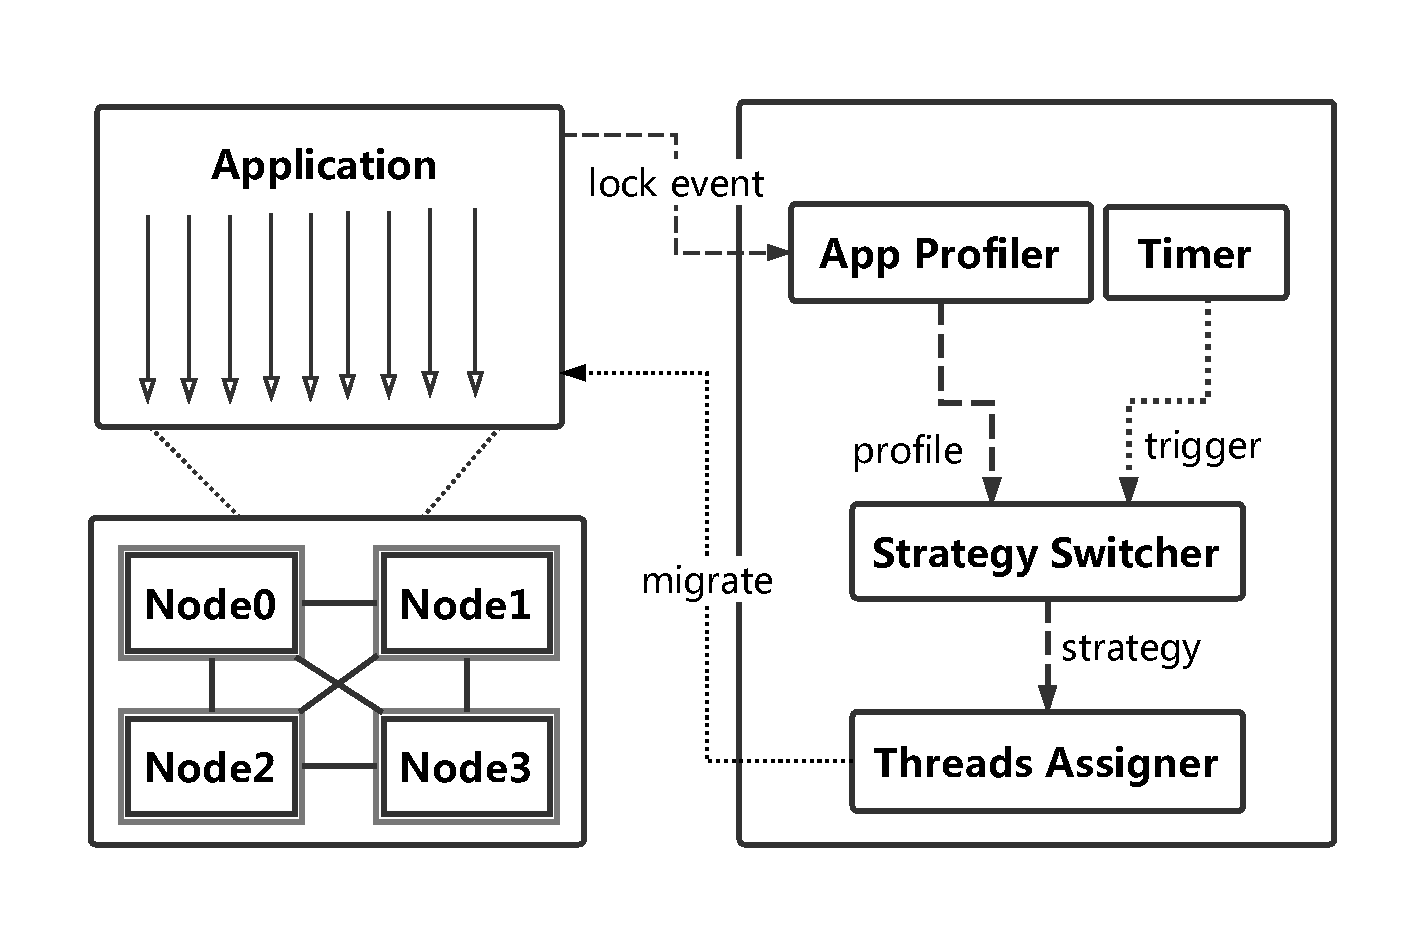
\includegraphics[width=5.6in]{archi.pdf}
	\caption{MSS的总体架构}
	\label{Fig:archi}
\end{figure}

\subsection{总体架构}
MSS的总体架构如图\ref{Fig:archi}所示。MSS逻辑上包含四个模块:应用分析器(application profiler)、计时器(timer)、策略转换器(strategy switcher)和线程调度器(threads assigner)。应用分析器负责监测分析应用的竞争状况,包括维护线程的分布,收集线程与锁相关的操作及更具锁事件流持续更新饱和点的值等。计时器负责产生定期的超时信号,该超时信号主要有两个功能:1)触发策略转换器生成新的线程放置策略;2)当应用有轮换的紧凑放置策略时触发线程调度器确定在合适的时间会被交换的候选线程。策略转换器在被计时器出发时负责根据当前的应用状态生成新的线程放置策略并且如果有必要的话切换到新的线程放置策略。线程调度器负责将新产生的线程放置策略应用到当前的应用程序中去,如果当前采用的是有轮换的紧凑策略还需要负责线程大的轮换。MSS的工作流程如算法\ref{algo:mss}所示,本章接下来的小节会详细介绍工作流程中的部分重要的考虑因素。

\begin{algorithm}
% \begin{algorithm}[H] % 强制定位
\caption{MSS 线程放置框架}
\label{algo:mss}
\begin{algorithmic}[1] %每行显示行号
\Require Cores\_per\_node:每个节点上的核数 每个节点上的线程数, Current:当前的线程放置策略 % 输入
\Repeat
\Comment{Every switching interval}
\State profile application to get number of threads(Threads) and saturation point(Saturation).
\If{$Threads\  \%\  Cores\_per\_node == 0$}
    \State $Nodes \gets Threads\  / \ Cores\_per\_node$
\Else
    \State $Nodes \gets Threads\  / \ Cores\_per\_node + 1$
\EndIf

\State $Average \gets Threads\  / \ Nodes$

\If{$Average\  >=\  Saturation$}
    \State $Placement \gets Restricted\_Even$
\Else
    \State $Placement \gets Compact\_With\_Shift$
\EndIf

\If{$Placement\  !=\  Current$}
    \State $Current \gets Placement$
    \State switch threads placement strategy to Current 
\EndIf

\If{$Current\  ==\  Compact\_With\_Shift$}
    \State perform shift
\EndIf

\Until{application terminates}
\end{algorithmic}
\end{algorithm}

\section{切换和轮换频率}
为了实现一个实际的MSS框架,我们需要为几个周期性的操作确定合适的时间间隔。首先我们需要确定一个合适的切换间隔(switching interval),即线程放置策略的更新间隔;其次为了有轮换的紧凑放置策略能够保证长期公平性,我们需要选择一个合适的轮换间隔(shifting interval),即在两个线程等价类之间交换线程的时间间隔。

\subsection{切换间隔}
我们用Linux的系统时钟(ualarm 函数)来生成定期的软中断,并且用连续两次软中断之间的时间间隔作为一个切换间隔。虽然较小的切换间隔能够根据应用中竞争状况的变化做出细力度的线程放置策略调整,但是过小的切换间隔会带来不必要的系统开销并且可能造成两种线程放置策略的过于频繁的切换进而带来额外的线程迁移代价,所以选择一个合适的切换频率非常重要。在MSS中我们将切换间隔作为一个配置参数,其默认值为(200ms),用户可以根据应用的实际状况对该参数进行配置,在我们的实验中200ms带来的系统开销可以忽略不记并且能够很好的适应应用竞争状况的变化。

\begin{figure}[t]
	\centering
	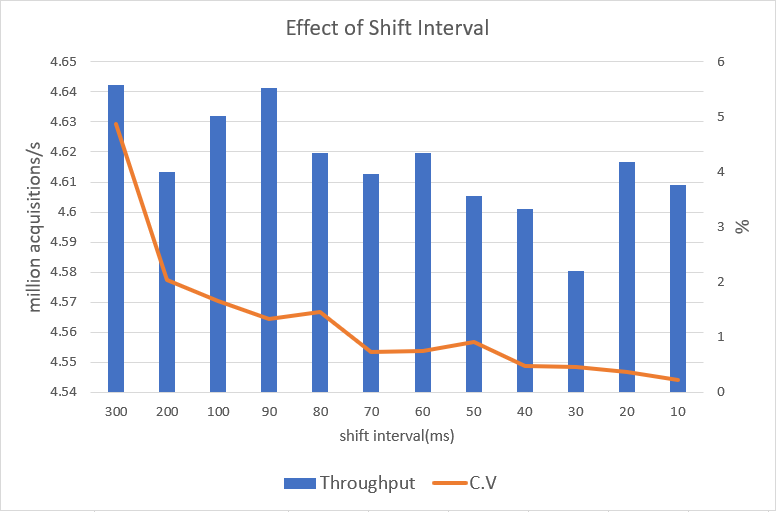
\includegraphics[width=5.6in]{shift-interval.PNG}
	\caption{轮换间隔对吞吐率和长期公平性的影响}
	\label{Fig:shift-interval}
\end{figure}

\subsection{轮换间隔}
轮换被用来弥补紧凑策略不能保证长期公平性的缺陷因而只有应用有轮换的紧凑策略时该参数才有意义。轮换间隔实际上时性能和长期公平性之间的一个折衷,较小的轮换间隔使得两个线程等价类之间更频繁的交换线程从而达到更好的长期公平性,但是线程迁移也会带来额外的系统开销比如造成缓存污染等从而对吞吐率产生影响。为了找到一个合适的轮换间隔,我们在Intel Xeon5上运行了stress\_one,我们给该应用配置了12个线程,并且应用了有轮换的紧凑放置策略。图\ref{Fig:shift-interval}显示了不同轮换间隔下的总吞吐率和长期公平性,其中我们用单个线程吞吐率之间的变异系数来衡量长期公平性,变异系数越小,长期公平性越好。不使用轮换策略时的吞吐率4639106 acquisitions/s,变异系数为64\%。从图\ref{Fig:shift-interval}中可以看出当轮换间隔大于10ms时吞吐率几乎不受影响(吞吐率损失在1\%以内),这主要是因为(1)线程迁移发生在关键路径之外;2)当很多线程激烈竞争同一个锁及其保护的数据时,大多数线程大多数时间并没有做有用的工作,所以线程迁移的代价并不会对吞吐率产生明显的影响。变异系数随着轮换间隔的减小而呈下降趋势,即轮换间隔越小,长期公平性呈越好的趋势。当轮换间隔小于等于50ms,变异系数恒小于1\%所以我们将50ms作为轮换间隔的默认值。

\section{应用分析}
应用分析器是是MSS竞争感知的关键,为了分析应用程序当前的竞争状态,分析器需要在每个切换间隔内维护或者收集以下三个方面的信息:
\begin{enumerate}
  \item 硬件配置信息,比如机器包含的NUMA节点数和每个节点上的计算核心数;
  \item 应用中当前的线程总数;
  \item 当前的饱和点的值;
\end{enumerate}
对于一个特定的机器来说,硬件配置信息是在应用运行之前就已知并且恒定不变的,所以我们将其存储在层级所的配置文件中。线程总数存储在变量\emph{contenders}中并且会在线程创建销毁的时候进行更新。

饱和点的值会随着程序的运行而变化所以只能在程序的运行过程中去评估。应用分析器通过取样每个线程的锁事件来评估饱和点的值,实验中我们发现饱和点的值对于锁事件的取样频率不是很敏感所以我们将取样频率设置为每个循环中每个线程一次。在每一个锁事件中,线程会将其拿锁,放锁及再次请求锁的时间戳记录在其私有内存(thread local memory)中。基于这三个时间戳,应用分析器可以得到关键区域长度实例cs和非关键区域长度ncs,并且计算出一个饱和点实例,即
\begin{equation}\label{Eq:saturationInstance}
     SatInstance = (ncs + cs) / cs
\end{equation}
如果这是第一次取样,那么我们将饱和点的值设为SatInstance,否则,为了更新饱和点的值,我们使用下述衰老机制(aging mechanism):
\begin{equation}
     Sat = Sat * \alpha + SatInstance * (1 - \alpha)
\end{equation}
其中$\alpha$是饱和点旧值的权重,在实际的实现中我们将$\alpha$的值设为
\begin{equation}
     \alpha = 1 - 1/contenders
\end{equation} 
从而使得每个竞争者为饱和点贡献相同的权重。更新完饱和点的值之后,这三个时间戳就不需要了所以他们所占用的内存空间可以被用来做下一次取样,因此应用分析的额外内存开销是可以忽略不计的。另外,饱和点的更新都发生在放锁之后所以只消耗计算资源而不会加长关键区域长度。

\section{生成放置策略}
MSS通过应用混合放置策略来利用单个策略的优势的同时避免其缺陷,所以根据具体的应用竞争状况确定合适的线程放置策略对于发挥混合策略的优势至关重要。正如前面章节讲到的,MSS偏好加强的平均放置策略,所以其生成线程放置策略的基本原则是如果当前的竞争状况下加强的平均放置策略能够同时保证高吞吐率和长期公平性则采用加强的平均放置,否则采用有轮换的紧凑放置。

具体来说,当被计时器出发时,策略转换器首先根据\emph{contenders}即硬件信息计算和分配能够保证每个线程都被放置到一个专用计算核心的最少需要的节点数,然后计算出平均每个节点上应该放置的线程数Avg,最后策略转换器按照公式\ref{Eq:policy}来生成新的线程放置策略:
\begin{equation}\label{Eq:policy}
strategy=
\begin{cases}
restricted\ even &\text{Avg >= $\lceil Sat \rceil$ + 1}\\
compact\ with\ shift &\text{Avg <= $\lfloor Sat \rfloor$ - 1}\\
current &\text{Otherwise}
\end{cases}
\end{equation}
其中current表示当前正在应用的线程放置策略,我们给Sat加一或减一来防止线程放置策略在加强的平均放置和有轮换的紧凑放置之间频繁抖动。如果新的线程放置策略与原先的不同,则线程调度器会根据新的线程放置策略来生成线程在节点间的目标分布,应用中的所有线程看到线程放置策略的变化后就可以根据其当前运行的位置和目标线程分布来决定迁移与否,下面的章节对其做详细介绍。

虽然MSS偏向于应用加强的平均放置策略,但是在应用刚开始运行的时候还是采用有轮换的紧凑放置策略因为一开始我们并不确定应用中的竞争是不是大到能是加强的平均放置策略保证高吞吐率。在应用开始运行之后就可以根据应用状态的变化来合理的选择最合适的线程放置策略了。

\section{线程调度}
MSS的线程调度器并不是系统调度器的延申,相反,线程调度策略是以一种分布式的方式由所有线程做出来的。每个线程根据其当前运行的位置和当前线程放置策略的目标线程分布决定要不要迁移到其他节点上去,因此为了达到最终的线程分布,每个线程必须知道其当前的运行位置和当前所有线程在相关节点间的分布。每个线程当前的位置可以很容易地通过汇编指令rdtscp得到;MSS在层级锁地数据结构中维护了一个位图(bitmap)来记录当前所有相关线程在节点间地分布。该位图事实上记录当前每一个计算核心是不是已经分配给了某个线程,所以也可以用来保证每个线程被放置到一个专用核上。当一个线程决定迁移时,它会首先通过在位图上设置相应地位来在目标节点上申请一个空闲核,然后通过在位图上擦出相应地位来释放当前核地所有权,最后迁移到目标节点上相应的核上去。虽然位图在应用程序中的所有线程之间共享,但是它的修改不需要锁来同步,因为修改发生在线程放锁时而没有两个线程会同时放锁。下面我们分别详细介绍加强的平均放置和有轮换的紧凑放置下的线程迁移决策。

\subsection{加强的平均放置}
当策略转换器切换到加强的平均放置或者有线程生成和销毁时,为了保持线程的平均放置,每个线程按照下述步骤来做出迁移决策,先计算出平均每个节点上应该放置的线程数average,然后将其与当前节点上的线程数比较,如果当前节点上的线程数较少或者正好等于average,那么该线程无需迁移;否则,该线程找到一个线程数少于average的相关节点或者有必要的话申请一个新的节点,然后迁移到目标节点上的一个可用核上去。

虽然上述操作都发生在关键区域之外,但是他们还是会消耗额外的计算资源,为了进一步减少额外计算资源的使用,MSS设置了一个标志变量need\_migrate来表示当前的线程分布是否需要通过进一步的线程迁移来满足加强的平均放置的要求。该标志变量一开始被设置为true并且在线程创建、迁移和销毁之后被更新,每个线程首先检查该变量的值,只有当其为true时才进行后续的操作,因而大多数的计算都能够被避免掉。此外,虽然need\_migrate是在所有线程之间全局共享的,更新它只会带了忽略不计及的最后一级缓存(last level cache)不命中,因为一般情况下切换到一个新的线程放置策略只需要很少的线程迁移,need\_migrate并不需要频繁地更新。
\subsection{有轮换的紧凑放置}
有轮换地紧凑放置通过两步来调度线程:1)按照紧凑策略来放置线程,从而所以线程被分为两个等价类,即所有放满线程地节点上地线程构成一个等价类,其余线程构成另一个等价类;2)定期按照循环赛(round-Robin)地方式从两个等价类中各选一个线程出来然后交换它们地运行位置,从而逻辑上所有线程形成一个圆圈并且每次超同一个方向移动一个位置,长期来看每个线程在每个位置运行了差不多相同的时间。第一步尽可能地保持了局部性从而能够提供高吞吐率;第二步抹平了线程间地吞吐率差异因而可以保证长期公平性。
\begin{figure}[t]
	\centering
	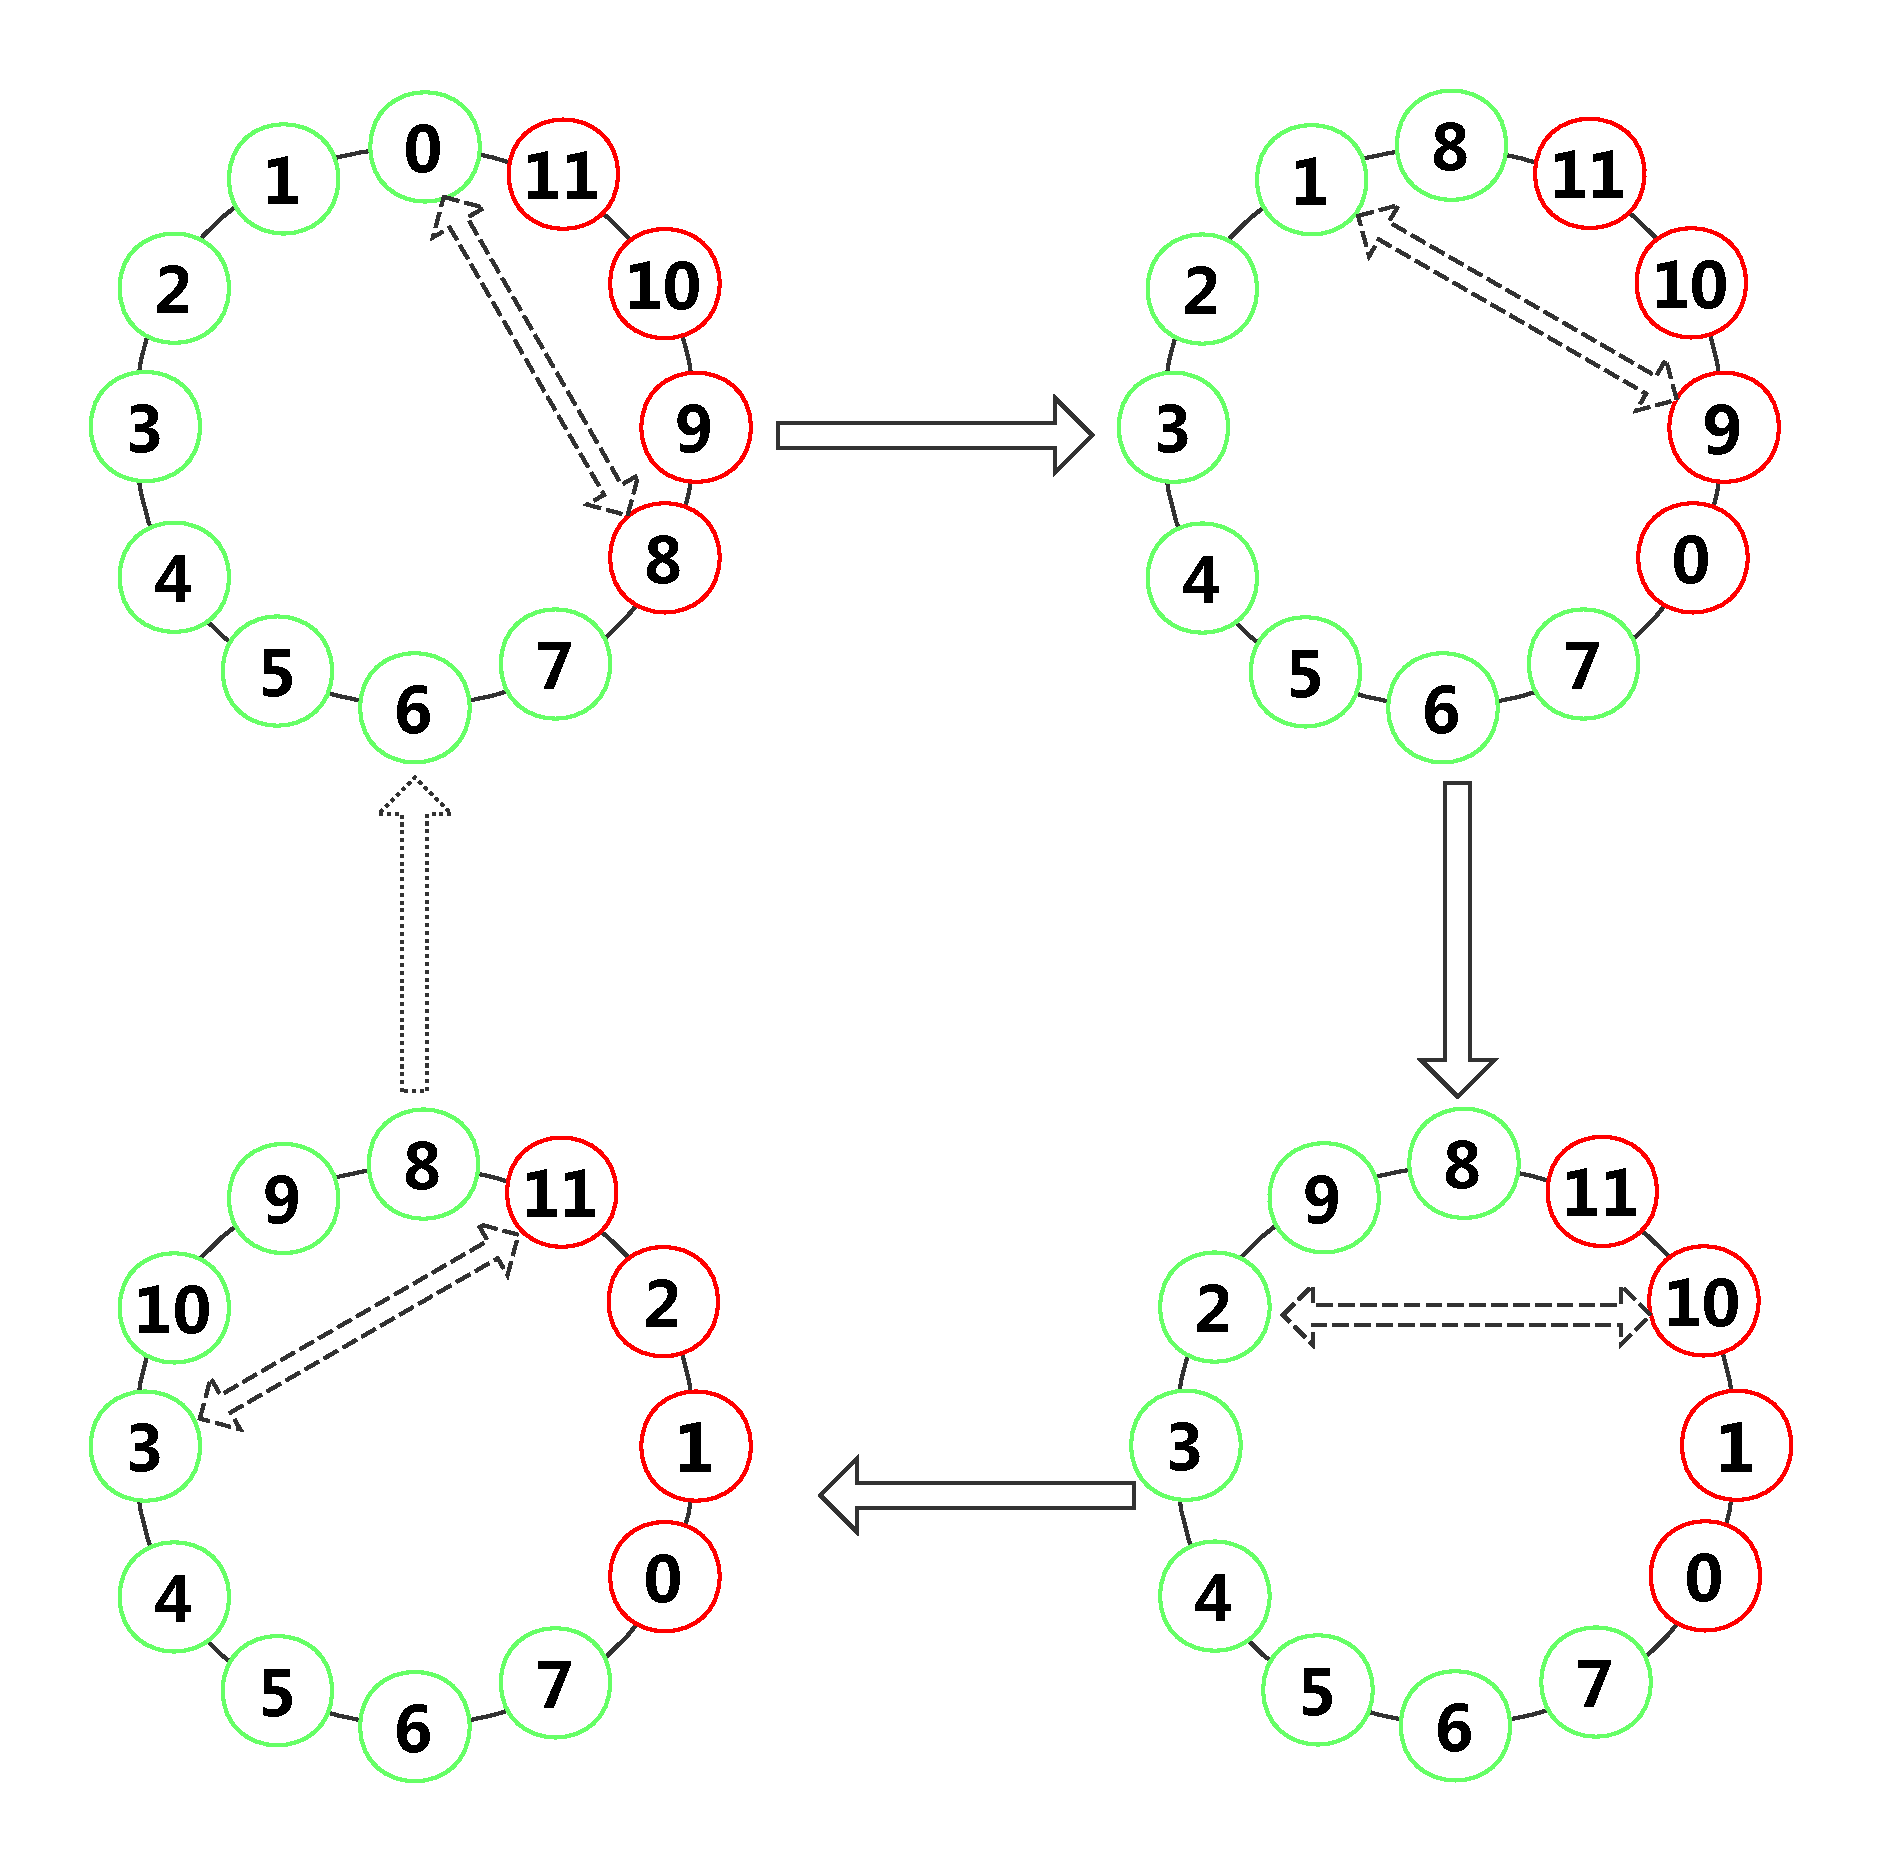
\includegraphics[width=5.6in]{shift.pdf}
	\caption{Shifting threads between equivalent groups}
	\label{Fig:shift}
\end{figure}

MSS用类似加强的平均放置的方式完成第一步地线程放置。为了完成第二步的线程定期轮换,我们将每个等价类中的线程各压入一个先进先出的队列,然后再每个轮换间隔内,线程调度器从每个队列的队首个弹出一个线程,交换其运行位置,并将其压入对方原先所在的队列的队尾。从长远来看,每个线程在每个等价类中待了差不多相同的时间,所以它们的吞吐率之间的差异被抹平而长期公平性也得到的保证。

图\ref{Fig:shift}展示了一个配置有12个线程的应用运行在两个节点上,每个节点有8个核的轮换示例。不同颜色的圆圈代表不同节点上的核,圆圈中的数字代表运行在其上的线程编号。第一步的放置操作之后,0至7号线程被放置一个节点上,剩下的4个线程被放置在另一个节点上。第一个轮换间隔之后,线程调度器交换了0号和8号线程;第二个轮换间隔之后,线程调度器交换了1号和9号的位置...,线程调度器重复上述操作,从长远来看,每个线程在每个节点上运行的时间差不多所以每个线程的吞吐率也差不多。

在具体的实现中,两个候选线程是在每个轮换间隔的超时信号发出时确定的,而具体的线程迁移则是在对应的候选线程放锁之后进行的,这样做的主要母的也是为了放置线程迁移加长关键路径的长度。为了避免在线程迁移的过程中将两个线程调度到同一个核上,我们要求跑在放满线程的节点上的候选线程先迁移到另外一个候选线程所在节点上的某个可以的核上,然后另外一个候选线程再迁移到该线程原来运行的位置。

\section{具体实现}
MSS的实现不需要修改内核调度器的代码,也不需要修改应用代码。MSS的全部功能是基于libslcok\cite{kashyap2017scalable}中的cstmcs锁实现的,上述设计中的所有修改,包括锁事件的取样、饱和点的更新、线程放置策略的生成以及线程的迁移等,都发生原有cstmcs锁的初始化、销毁或者拿锁、放锁函数中。

\begin{figure}[t]
	\centering
	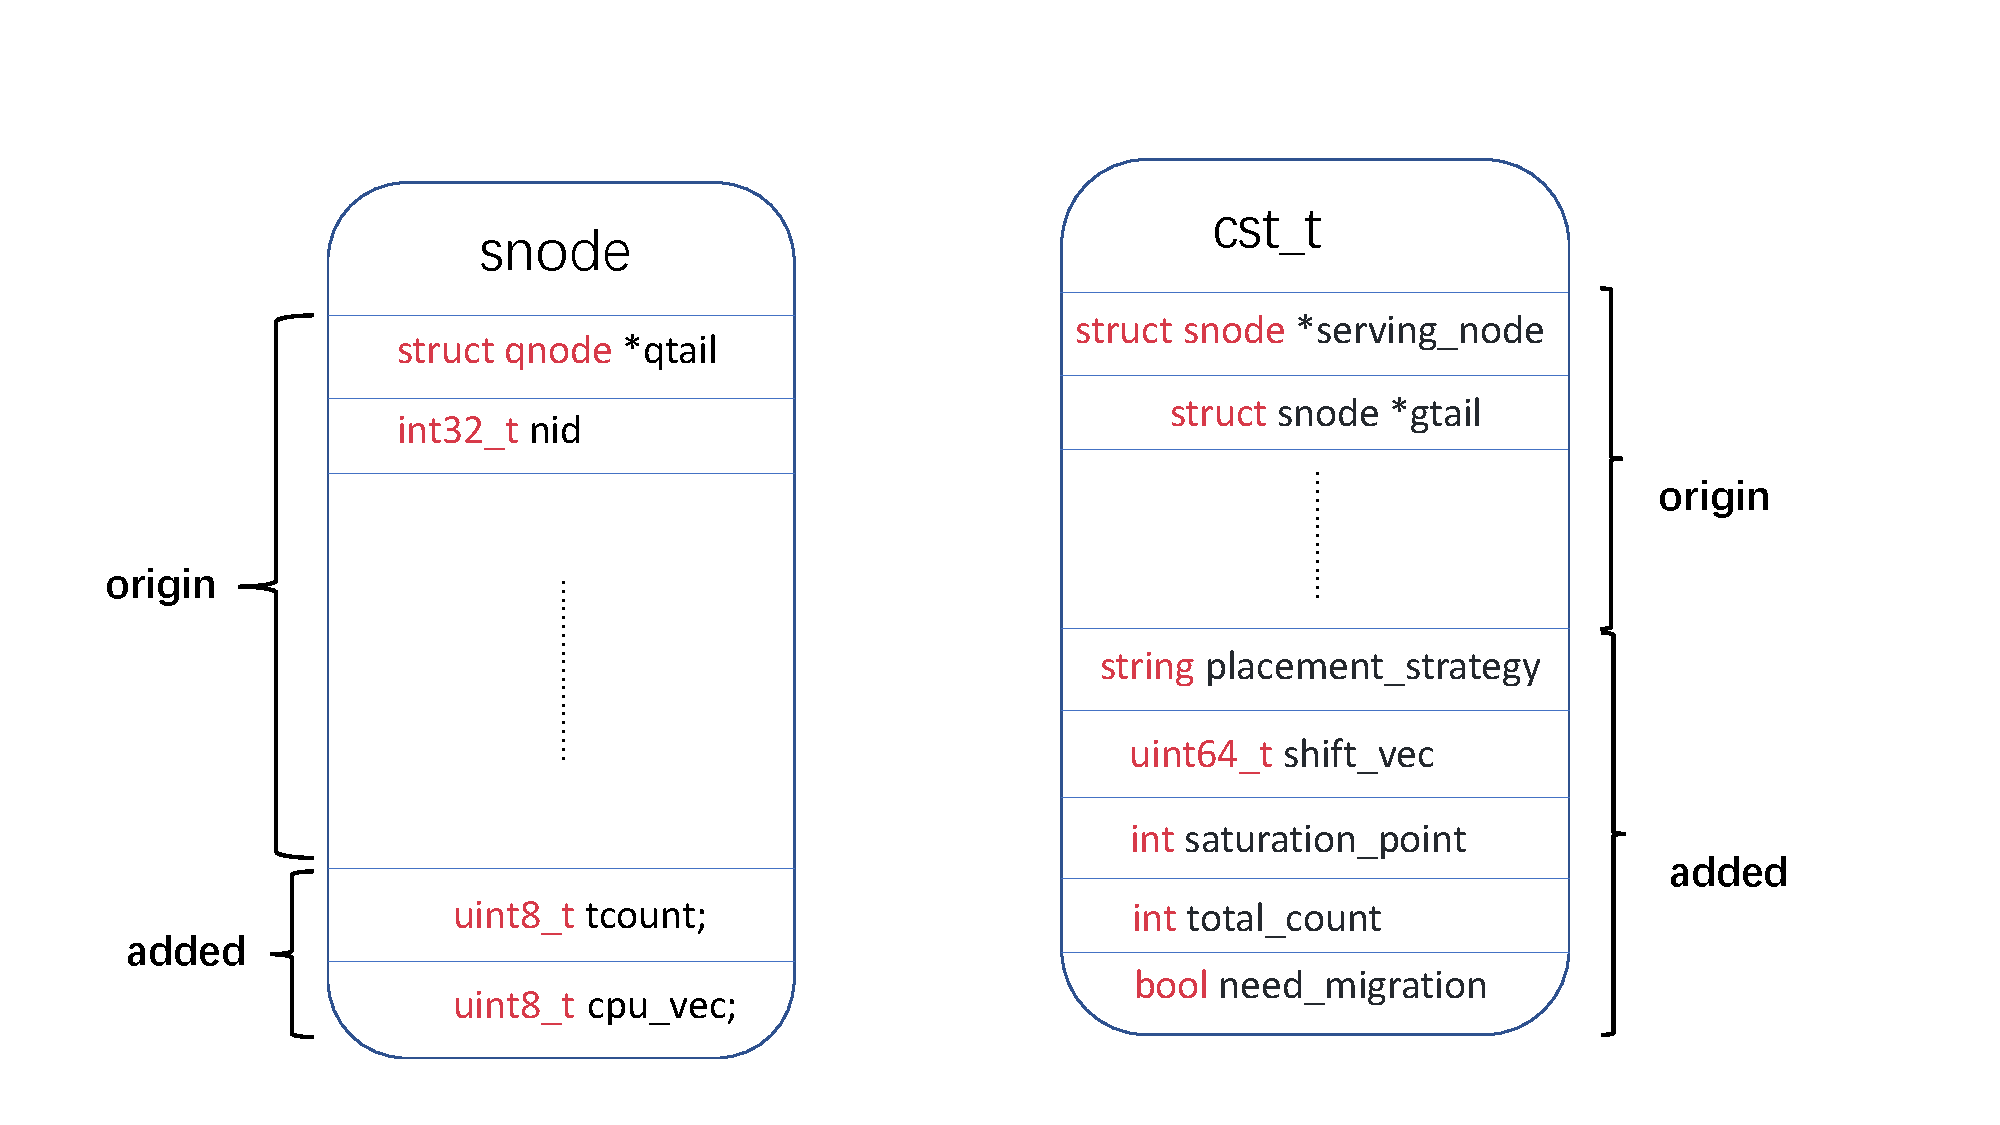
\includegraphics[width=5.6in]{struct.pdf}
	\caption{Modification on the original cstmcs lock structure}
	\label{Fig:struct}
\end{figure}

为了实现MSS,我们首先在cstmcs中的cst\_t(代表cstmcs锁)和snode(代表每个NUMA节点)等结构体加了一些新的数据成员,如图\ref{Fig:struct}所示,修改后每个snode主要包含以下数据成员:
\begin{itemize}
\item qtail:节点对应的本地MCS锁的tail指针;
\item nid:节点的编号;
\item tcount:节点上运行的线程数;
\item cpu\_vec: 节点上每个核的状态(是否可用)。
\end{itemize}
其中tcount的更新发生在每个线程初始化和销毁其对应的MCS锁记录(entry)时;cpu\_vec的更新发生在每次线程迁移前后。
修改后的cst\_t包含以下数据成员:
\begin{itemize}
\item serving\_node:当前全局锁锁在的节点;
\item gtail:全局MCS锁对应的tail指针;
\item shift\_vec:下个shift周期内交换位置的线程对;
\item saturation\_point: 饱和点;
\item total\_count:总线程数;
\item need\_migration:当前线程分布是否满足放置策略的要求;
\item placement\_strategy:当前应用的线程放置策略;
\end{itemize}
其中shift\_vec在每个轮换间隔的超时信号发生时由处理该信号的线程通过两个先进先出的队列来更新,具体如上节所述;saturation\_point在每次锁事件的取样之后更新,具体来说,我们在线程拿锁、放锁、请求锁的时候分别记录三个时间戳,然后根据这些时间戳来更新saturation\_point,具体的更新算法如上节有详细描述;total\_count的更新与每个节点上的tcount的更新同步;线程每次迁移之后会判断当前的线程分布是否满足当前线程放置策略的要求,进而更新need\_migration。

切换间隔和轮换间隔都是由同一个计时器产生的,为了用单个计时器满足两个周期性操作的要求,我们要求切换间隔时轮换间隔的整数倍,这也符合实际的情况。该计时器是用ualarm函数实现的,ualarm函数会产生周期性的SIGALAM信号并将该信号发送给对应进程,然后我们用signal函数注册了相应的处理函数来处理SIGALAM信号。具体来说,如果该信号只表示一个轮换间隔结束,那么该处理函数只从当前的进程中选出两个候选者然后更新shift\_vec即可,否则该信号还表示一个切换间隔的结束,此时该处理函数还需要根据total\_count和saturation\_point来生成一个新的线程放置策略并更新placement\_strategy。
\begin{lstlisting}[language={C}, caption={注册信号处理函数}]
void ( *signal( int sig, void (* handler)( int )))( int );
\end{lstlisting}

获取形成的当前运行位置(哪个核上)及记录事件的时间戳都是通过RDTSCP((Read Time Stamp Counter))机器指令来实现的。RDTSCP可以读取当前运行的CPU的时间戳计数寄存器TSC(Time Stamp Counter)的值,并将其高32位存入EDX寄存器,低32位存入EAX寄存器,同时处理器的ID。现有的C/C++编译器不直接支持使用RDTSC指令,所以我们使用需用内联汇编的方式对其进行访问,如下所示
\begin{lstlisting}[language={C}, caption={通过内联汇编来使用RDTSCP指令}]
    uint32_t a, d, c;
    //rdtscp---Read Time-Stamp Counter(EDX:EAX) and Processor ID(ECX)
    __asm__ volatile("rdtscp" : "=a"(a), "=d"(d), "=c"(c));
    c = (c & 0xFFF);
\end{lstlisting}

MSS通过线程迁移来完成相关的线程放置策略,但是我们并没有修改Linux内核代码,所以不能直接利用Linux调度器来完成线程迁移。具体实现中我们利用了Linux内核提供的并且被GNU C定义的相关接口来设置线程与核的亲和性进而通过Linux调度器来间接完成线程迁移。具体来说,我们用到了CPU\_SET函数和cpu\_set\_t类型。cpu\_set\_t是一个位集合(bitset),其中每个比特代表一个CPU,通过cpu\_set\_t设置CPU掩码,然后调用CPU\_SET设置线程和CPU的亲核性就可以完成线程的间接迁移。

\section{讨论}
大多数应用的关键区域执行时间非常短,而且关键共享数据也很少,所以锁本身所占的内存空间及锁传递的开销对于整体性能的影响可能会非常大,在现有高性能锁实现上的不恰当的微小修改都可能造成原有锁的性能的极大损失。MSS在实现过程中充分考虑了各种实现方法对原有cstmcs锁的内存使用及锁传递效率的影响并且采用了多种机制来尽可能地避免这些不利影响。

如图\ref{Fig:struct}所示,MSS中只增加了几个变量,所以内存方面的开销可以忽略不计。为了避免额外操作加长关键路径我们主要采用了以下几个措施:1)额外操作尽可能放在放锁之后,比如锁迁移、相关变量的更新等,从而避开关键路径,利用线程自旋CPU空转的的时间做有益的操作;2)延迟迁移,在shift机制中,将候选线程对的选择和候选线程对的位置交换解耦,即轮换超时信号触发时只做候选线程对的选择,而候选线程对的位置交换(线程迁移)还是在相关线程放锁之后进行。此外,我们还采取了多种措施来尽可能减少额外操作,比如通过need\_migration来避免线程每次放锁之后都通过大量计算来判断当前线程的分布是不是达到当前线程放置策略的要求。另外,全局共享变量的频繁更新会造成大量的缓存一致性操作,从而对性能和可扩展性等方面造成不利影响,MSS中使用的全局共享变量主要是cst\_t中新加的几个成员,通过前边章节的分析可以看出这些成员的更新频率很低,所以不会对原有锁的性能造成明显影响。
